\section{Conception — PIM}

\begin{figure}[p]
\centering
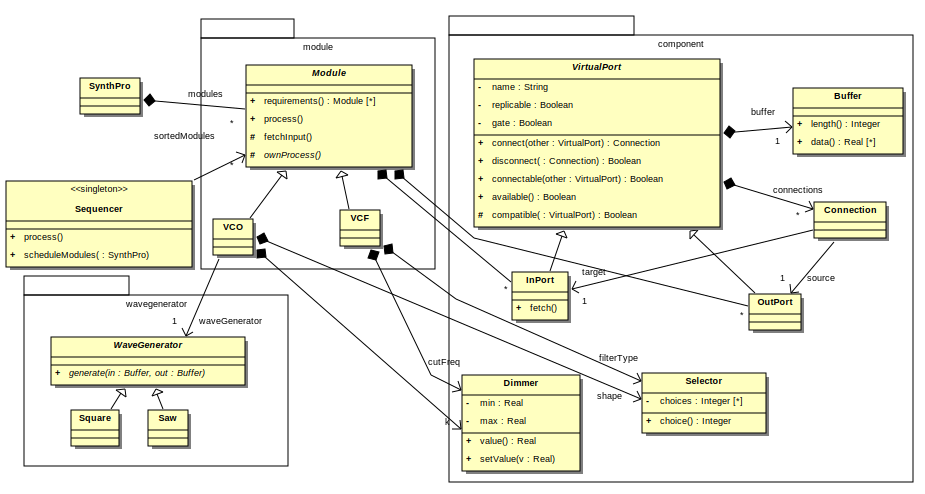
\includegraphics[width=23cm,angle=90]{../img/ps/business-pim-light.pdf}
\caption{Classes principales de la partie métier}
\label{pim-class}
\end{figure}

La figure \ref{pim-class} présente la majeure partie de notre modèle de la composante
métier du système. La classe \verb!SynthPro! représente le
synthétiseur, il contient un ensemble de modules lesquels
contiennent des ports permettant de créer des connections entre
eux.

\subsection{Moteur}

La classe \verb!Sequencer! gère le \emph{dataflow}~: l'opération
\verb!scheduleModules! trie le graphe des modules contenus dans le
synthétiseur en fonction de leurs dépendances, et l'opération
\verb!process! appelle l'opération du même nom sur chaque élément
de la liste de modules triée, de telle sorte que chacun réalise son
traitement.

Le tri des modules est un simple tri topologique,
réalisé par un parcours en profondeur du graphe de modules~: une
première passe recherche les modules «~puits~» (ceux qui ne
possèdent pas de port de sortie), puis \emph{via} une opération
\verb!requirements! (de la classe \verb!Module!) qui retourne la
liste des modules connectés aux ports d'entrée d'un module, le
séquenceur détermine un ordre d'exécution possible pour satisfaire
toutes les dépendances. L'algorithme ignore les cycles (il ne
visite pas deux fois un même nœud).

Une classe \texttt{Clock} (non représentée sur le diagramme) appelle périodiquement,
en tâche de fond, l’opération \texttt{process} du séquenceur.

\subsection{Modules}

Le \emph{package} \verb!module! contient l'ensemble des modules (ne
sont représentés sur la figure \ref{pim-class} que le VCO et le VCF). La classe
mère, \verb!Module!, contient l'opération \verb!process! dont
l'implémentation appelle \verb!fetchInput! (qui récupère les données des ports connectés aux ports d’entrée du module) puis \verb!ownProcess!.
Cette dernière est abstraite (patron de conception
\emph{Template Method}), laissant le soin à chaque module de
définir sont traitement spécifique (par exemple appliquer un filtre sur le signal).

\subsection{Composants}

Le \emph{package} \verb!components! définit les classes
représentant les éléments constitutifs des modules, en particulier
les ports. Les ports sont les composants qui permettent de relier
les modules entre eux, et il est fréquent de vouloir relier une
même sortie aux entrées de plusieurs modules (démultiplexage) ou
connecter les sorties de plusieurs modules à l'entrée d'un même
module (mixage). Pour cela nous avons introduit la notion de port
«~virtuel~»~: un tel port peut se répliquer à l'infini, permettant
d'être connecté à plusieurs autres ports et réalisant
automatiquement le travail de démultiplexage ou de mixage (cf. explication en section \ref{ports-virtuels}). Il est
défini par la classe \verb!VirtualPort!. L'attribut
\verb!replicable! indique si un port peut effectivement se
répliquer et les opérations \verb!connect! et \verb!disconnect!
créent et suppriment des connexions. Nous avons également introduit
un attribut \verb!gate! permettant de différencier les ports ayant
une fonction de \emph{gate} (déclencheur) des autres. Les ports de
sortie de type \emph{gate} sont plus susceptibles d'être connectés
à des ports d'entrée de type \emph{gate}, mais le système
n'interdit pas de les connecter sur les autres ports.

La classe \verb!InPort! hérite de \verb!VirtualPort!, elle définit
la notion de port d'entrée et contient une opération
supplémentaire, \verb!fetch!, qui copie les données des ports de
sortie auxquels elle est reliée dans son propre \emph{buffer} (elle
réalise le mixage en faisant la somme de toutes ces données).

Enfin, les classes \verb!Dimmer! et \verb!Selector! définissent des
composants permettant d'ajouter des réglages aux modules, sous la
forme d'un potentiomètre (permettant d'indiquer une valeur dans un
intervalle donné) ou d'un «~sélecteur~» (permettant de choisir une
valeur dans un ensemble fini donné), respectivement.

Le \emph{package} \verb!wavegenerator! contient des classes
définissant des générateurs de signaux de formes différentes~:
carrée, triangle, etc. (patron de conception
\emph{Strategy}). Un \emph{package} analogue, \verb!filter! (non
représenté sur le schéma) contient les différentes stratégies de
filtres (passe-bas, passe-haut, etc.) utilisables par les modules.

\subsection{Interface utilisateur}

\subsubsection{Modèle PAC}

Le modèle PAC est utilisé pour rendre le logiciel interactif~: pour
chaque classe de la partie métier devant être représentée dans
l'interface utilisateur, une classe de contrôle et une classe de
présentation sont créées. La figure \ref{pacdimmer-pim} montre un tel découpage pour
les potentiomètres (classe \verb!Dimmer!).

\begin{figure}[h]
\centering
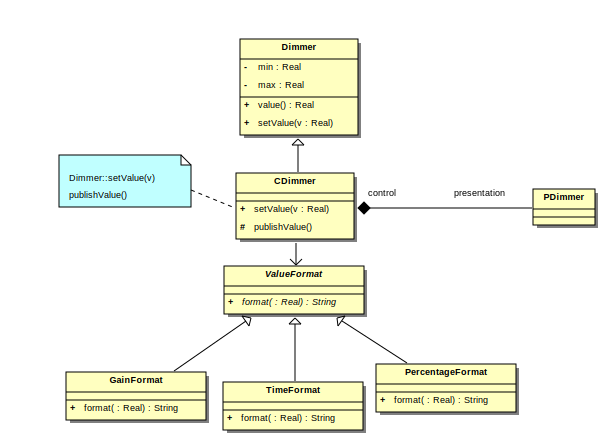
\includegraphics[width=16cm]{../img/ps/pacdimmer-pim.pdf}
\caption{Modèle PAC appliqué à la classe Dimmer}
\label{pacdimmer-pim}
\end{figure}

Nous avons choisi de réaliser un \emph{Proxy} par héritage (plutôt
que par délégation) pour définir le contrôle, d'une part parce que
c'est plus pratique à écrire\footnote{Nous ne redéfinissons que les
opérations à «~intercepter~».} et d'autre part parce que cela permet
d'intercepter également les appels internes de l'abstraction\footnote{Avec
une solution par délégation, si l'abstraction appelle une de ses
propres opérations elle n'est pas interceptée par le
proxy.}, en dépit du fort couplage que cela introduit entre les
composants d'abstraction et de contrôle.

Dans le cas de la classe \verb!Dimmer!, nous voulons pouvoir
personnaliser l'affichage en fonction de l'interprétation de la
valeur du potentiomètre. Pour certains modules cette valeur
représente une fréquence, pour d'autres une amplification, ou
encore un délai. Pour cela, le contrôle est associé à une fonction
de mise en forme (réifiée par la classe \verb!ValueFormat!),
chargée de \emph{mapper} une valeur numérique vers une
représentation sous forme de chaîne de caractères. Ainsi le
contrôle du module \verb!VCO! configure le contrôle du réglage
\verb!k! de la fréquence du signal à générer en lui fournissant une
fonction de \emph{mapping} affichant la valeur en Hertz de la
fréquence. Chaque contrôle de module fait de même avec chacun de
ses potentiomètre pour personnaliser leur affichage. De cette
manière, les informations sur la façon de présenter ces valeurs ne
polluent pas l'abstraction.

\subsubsection{\textit{Drag and drop}}

\begin{figure}[p]
\centering
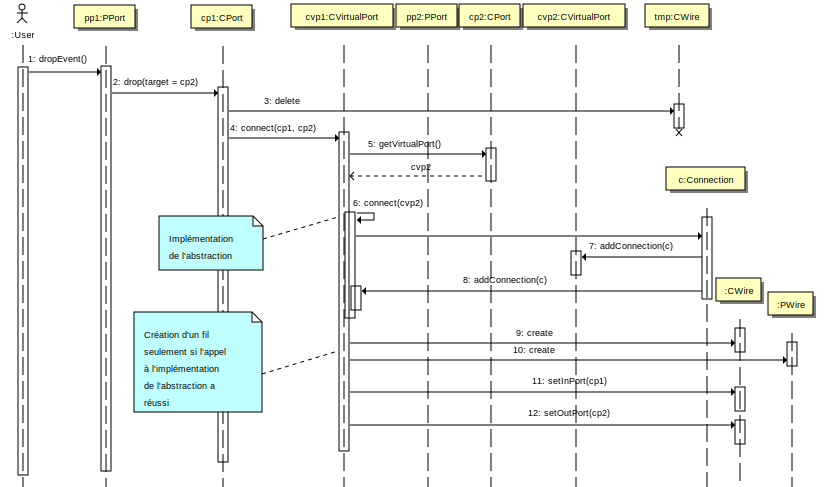
\includegraphics[width=23cm, angle=90]{../img/ps/drop-sequence.pdf}
\caption{Diagramme de séquence du drop}
\label{drop-sequence}
\end{figure}

La figure \ref{drop-sequence} illustre les échanges entre les composants lorsque
l'utilisateur termine une opération de \emph{drag and drop} reliant
un port d'un module à un autre pour les connecter.

Les classes \verb!CPort! et \verb!PPort! ont été ajoutées
uniquement pour les besoins de l'interface utilisateur et ne
correspondent pas à des classes dans l'abstraction, elles
représentent la notion de port où l'utilisateur peut brancher des
connexions (un \verb!VirtualPort! peut contenir plusieurs ports).
De même les classes \verb!CWire! et \verb!PWire! représentent la
notion (graphique) de fil et n'ont pas d'équivalent côté abstraction.

(1) L'événement \emph{drop} est capté par la présentation du port
source (objet \verb!pp1!) qui (2) transmet l'information à son
contrôle, \verb!cp1!, en lui indiquant le contrôle du port cible
\verb!cp2! (celui au-dessus duquel l'utilisateur a relâché la
souris, quand il ne la relâche pas dans le vide). (3) Le contrôle
\verb!cp1! supprime le fil qui était créé temporairement durant le
\emph{drag and drop} puis (4) transmet l'ordre au contrôle de son port
virtuel \verb!cvp1! d'établir une connexion entre les deux ports.
(6) La connexion est réalisée en appelant l'opération \verb!connect! de
l'abstraction (7, 8), et, selon son résultat (succès ou échec), un fil est
créé entre les deux ports (9).
